\documentclass{../industrial-development}
\graphicspath{{03-user-interface-design/}}

\title{Проектирование пользовательских интерфейсов}
\author{Лагутина Ксения Владимировна, ИТ-21 МО}
\date{}

\begin{document}

\begin{frame}
  \titlepage
\end{frame}

\begin{frame}{План лекции}
  \tableofcontents
\end{frame}

\section{Задача проектирования пользовательских интерфейсов}

\begin{frame} \frametitle{Основные цели интерфейса}\rmk{Точек на слайдах быть не должно!}
  \begin{definition}
    \alert{Пользовательский интерфейс} "--- это набор программных и \rmk{Если предлог повис на предыдущей строке, ставьте неразрывный пробел} аппаратных средств, обеспечивающих взаимодействие пользователя с компьютером.
  \end{definition}
  
  \begin{itemize}
   \item Интерфейс в первую очередь ориентирован на нужды пользователей.
   \item Интерфейс должен быть простым и понятным.
   \item При проектировании интерфейса не стоит полностью полагаться на <<промышленные стандарты>>.
  \end{itemize}
\end{frame}

\lecturenotes

Пользовательский интерфейс "--- это набор программных и аппаратных средств, обеспечивающих взаимодействие пользователя с компьютером~\cite{Bauman}.

Уже из определения становится очевидно, что разработка интерфейсов должна быть ориентирована на нужды пользователей. Первым шагом в этом направлении является стремление узнать своего пользователя. Прежде чем приступать к разработке самой программы или пытаться учесть различия между отдельными пользователями, разработчики интерфейса могут облегчить свой труд, сосредоточив внимание на том, что является общим для всех людей с точки зрения требований к интерфейсу.

После завершения этой стадии разработчики определяют, насколько будет отличаться интерфейс для различных групп пользователей, и ищут оптимальный варианта, который будет удовлетворять широкому диапазону требований пользовательских задач. Однако этот первый важный шаг, во время которого проект интерфейса приводится в соответствие с общими законами психологии, в процессе разработки обычно пропускается. Разработчики интерфейсов предпочитают не задумываться об этом и больше полагаются на так называемые <<промышленные стандарты>>. В результате все широко используемые сегодня модели интерфейсов построены без учета закономерностей мышления и поведения человека.

Качественное программное обеспечение должно быть простым и понятным, своим безупречным поведением показывая нам, что его создатели больше работали над удобством использования, нежели над привлекательным внешним видом своего продукта.~\cite[с.~5--6]{Raskin}

\begin{frame} \frametitle{Разработка интерфейса как часть цикла разработки ПО}
  \begin{itemize}
  \item Интерфейс проектируется на начальных стадиях разработки.
  \item Дальнейшая разработка продукта зависит от интерфейса.
  \item На каждом шаге цикла разработки интерфейс может быть изменен.
  \end{itemize}
  
  \begin{block}{}
    Пользовательская оценка продукта в значительной степени зависит от интерфейса!
  \end{block}
\end{frame}

\lecturenotes

Интерфейсом удобнее всего заниматься именно на начальных стадиях разработки. И если специалисты по интерфейсам привлекаются уже после того, как программное обеспечение спроектировано и определены его инструменты или когда разработка программы уже почти завершена, то их рекомендации могут потребовать переделки всей выполненной работы, что, очевидно, потребует больших затрат. Когда бюджет проекта уже исчерпан и рабочий план почти завершен, перспектива отказа от большей части или даже всего дизайна и готового кода, конечно, не может вызвать энтузиазма у менеджеров проекта. 

Определив задачу, для которой продукт предназначен, сначала спроектируйте интерфейс, после чего приступайте к его реализации. Это повторяющийся процесс. Определение задачи будет меняться во время разработки интерфейса. Поэтому весь процесс разработки продукта будет проходить в соответствии с изменениями в задаче продукта и его интерфейсе. Здесь необходимо стремиться к максимальной гибкости. На первом этапе разработки следует определить, что именно должен сделать пользователь для получения того или иного результата и как система должна отвечать на каждое его действие. Пользователи не задумываются над тем, как устроена машина, пока она справляется со своими задачами. Для пользователей важнее всего удобство и результаты. Но все, что они видят, "--- это интерфейс. Другими словами, с точки зрения потребителя именно интерфейс является конечным продуктом.~\cite[с.~7--8]{Raskin}

\section{Этапы разработки пользовательского интерфейса}

\subsection{Определение функциональности системы}

\begin{frame} \frametitle{Определение функциональности системы}

  \begin{block}{}
    \rmk{Двусмысленная фраза:} Функциональность продукта определяет интерфейс. Продумывайте ее \rmk{её} на несколько версий вперед!
  \end{block}
  
  \begin{block}{Способы определения функциональности}
    \begin{itemize}
    \item Анализ целей пользователей
    \item Анализ действий пользователей
    \end{itemize}
  \end{block}
\end{frame}

\lecturenotes

На первом этапе разработки продукта необходимо определить функциональность будущей системы. Это исключительно важный этап, поскольку именно функциональность будет определять весь интерфейс.

Очень важно понимать, что практически невозможно убрать из уже продающейся системы какие-либо функции. Имеющиеся пользователи обычно с исключительной неохотой переучиваются для использования новых функций взамен прежних. Это значит, что ненужная функция системы будет кочевать из версии в версию, раздувая размеры программы, снижая надежность и быстродействие, и, что более важно, ухудшая интерфейс (при этом и длительность разработки возрастает). Так что оптимальным вариантом работы почти всегда является проектирование функциональности сразу на несколько версий вперед.

Традиционно требования к функциональности исходят от отдела продаж или от его аналога. Такие требования имеют два источника, а именно жалобы имеющихся клиентов и системы конкурентов. К сожалению, оба эти источника сомнительны. Всегда может оказаться, что желание клиента получить новую функцию обусловлено не реальной потребностью в ней, но собственно концептуальными проблемами системы. Системы же конкурентов страдают как от такого же непонимания проблемы, так и от множества других причин. Это значит, что прислушиваться к сторонним требованиям к системе, безусловно, следует, но рассматривать эти требования нужно не как директивы, но как признаки общего неблагополучия.

Как определить нужную функциональность? Существуют два основных способа, а именно анализ целей и анализ действий пользователей. Эти способы фактически не конфликтуют друг с другом, более того, в процессе определения функциональности желательно использовать оба~\cite[с.~111--112]{Golovach}.

\begin{frame} \frametitle{Анализ целей пользователей}
  \begin{block}{Основная идея анализа}
    Пользователям нужны результаты работы продукта, а не сам продукт.
  \end{block}
  \begin{block}{Результат анализа}
    В результате должна быть сформулирована основная функциональность продукта без упоминания конкретных деталей.
  \end{block}
\end{frame}

\lecturenotes

Идеей, лежащей в основе данного метода, является простое соображение, гласящее, что людям не нужны инструменты сами по себе, нужны лишь результаты их работы. Никому не нужен текстовый процессор "--- нужна возможность с удобством писать тексты. Никому не нужна программа обработки изображений "--- нужны уже обработанные изображения. Это значит, что сами по себе функции никому не нужны и не важны. Людям нужно средство вообще, делающее возможным выполнять какую-либо работу.

Разницу подходов к выбору функциональности в такой системе удобно проиллюстрировать на примере тостера. Стандартный подход, при котором функции выбираются фактически произвольно, в лучшем случае приведет к такому заданию:<<Нужен ящик с узкой прямоугольной дыркой и нагревателем внутри>>.

Анализ целей пользователя приведет к другой формулировке: <<Нужен поджаренный хлеб. Похоже, что проще всего добиться этого созданием ящика с дыркой по форме куска хлеба и нагревателем внутри. С другой стороны, похоже, что этот способ не единственный>>.

Второй вариант при полном развитии этого метода может привести не только к созданию тостера, но и также и ростера --- устройства, в котором можно поджаривать не только хлеб.

Главное же другое. Ни в коем случае нельзя дать обмануть себя ненужной конкретикой, т. е. описанием того, какова должна быть будущая функциональность. Как правило, одного и того же результата можно добиться несколькими разными способами, при этом важно не только реализовать какой-либо способ, но и выбрать лучший. Анализ целей пользователя как раз и позволяет избежать ненужной конкретики.

Результатом этого процесса должен являться список целей, например, для тостера финальный список целей должен выглядеть очень просто: <<Должен поджаривать мелкие предметы, преимущественно хлеб>>.

После того, как истинные цели пользователей установлены, приходит время выбирать конкретный способ реализации функции, для чего используется второй метод~\cite[с.~112--113]{Golovach}.

\begin{frame} \frametitle{Анализ действий пользователей}
  \begin{block}{Основная идея анализа}
    Изучайте поведение людей, пользующихся аналогичными инструментами.
  \end{block}
  \begin{block}{Результат анализа}
    В результате должна быть определена функциональность и способы ее реализации.
  \end{block}
\end{frame}

\lecturenotes

Достижение почти всех целей требует от пользователей совершения определенных действий. В сколько-нибудь сложных интерактивных системах сами по себе выбранные стратегии действий влияют на требования к функциональности.

Возвращаясь к примеру с тостером, можно указать, что помимо возможности поджаривать хлеб он должен включаться и выключаться, более того, он должен быть устроен таким образом, чтобы его можно было удобно мыть. С другой стороны, возможно, что тостер можно сделать так, чтобы он не требовал мойки, в этом случае функция становится лишней. Разумеется, взаимодействие человека с тостером очень просто, здесь можно дойти до всего чисто логическим анализом. В компьютерных же системах взаимодействие обычно многократно сложнее, при этом логический анализ не всегда дает достаточно полный и точный результат.

Единственным выходом является наблюдение за людьми, выполняющими свою задачу, пользуясь уже имеющимися инструментами, а именно системами конкурентов (если они есть) и предметами реального мира. Неплохим источником материала для анализа часто служит даже не наблюдение за людьми, но анализ результатов их работы "--- если оказывается, что результат работы практически не зависит от используемого инструмента, это значит, что нужна только та функциональность, которая оказала воздействие на результат (т. е. функции, которыми никто не воспользовался, не нужны). Тут очень важно избежать эгоцентризма. Очень трудно отказаться от мысли <<если это нужно мне, это нужно и многим>>. Возможно, что и нужно. А возможно, что и нет. Единственным же способом проверить, нужна функция или нет, является наблюдение за пользователями и анализ их действий.

Кроме того, обычно есть несколько разных способов реализации функции. Анализ действий пользователей как раз и позволяет определить, какой именно способ следует предпочесть~\cite[с.~113--114]{Golovach}.

\subsection{Создание пользовательских сценариев}

\begin{frame} \frametitle{Сценарии использования}
  \begin{definition}
    \alert{Пользовательские сценарии} "--- это спецификация взаимодействия пользователей с системой в конкретных случаях.
  \end{definition}
  
  \begin{block}{Преимущества сценариев}
   \begin{itemize}
    \item Оптимизация продукта.
    \item Активное участие разработчиков на ранних этапах проектирования.
    \item Вклад в будущее тестирование.
    \item Создание сценариев не требует значительных затрат.
  \end{itemize}
  \end{block}
\end{frame}

\lecturenotes

Сценарии использования дают разработчикам структурированный способ учета требований к поведению системы. Они специфицируют, как пользователи взаимодействуют с системой. Цель создания сценариев "--- написать словесное описание взаимодействие пользователя с системой, не конкретизируя, как именно проходит взаимодействие, но уделяя возможно большее внимание всем целям пользователей. Количество сценариев может быть произвольным, главное, что они должны включать все типы задач, стоящих перед системой.

Основные достоинства сценариев:

Их создание побуждает разработчиков учитывать характеристики предполагаемых пользователей, их задачи и окружающую среду. Это приводит к лучшему пониманию устройства проектируемой системы, побуждая сразу же оптимизировать будущее взаимодействие. Дело в том, что на таких сценариях очень хорошо заметны ненужные шаги. Понятно, что от этих ненужных этапов смело можно избавиться уже на этой, весьма ранней, стадии проектирования.

При использовании этот метода разработчики будут активно вовлечены в написании сценариев, что значительно облегчает их дальнейшую работу над системой.

Сценарии являются удобным инструментом тестирования как интерфейса, так и функциональности продукта.

Генерация сценариев не требует больших затрат ресурсов~\cite[с.~116]{Golovach}~\cite{Usabilitynet-scenarios}.

\begin{frame} \frametitle{Метод создания сценариев}
   \begin{enumerate}
    \item Определите пользователей и их контекст.
    \item Декомпозируйте задачи пользователя.
    \item Опишите схему взаимодействия пользователя и системы.
    \item Оцените время разработки и критерии завершенности продукта.
   \end{enumerate}
   
   \begin{block}{}
    Для гибкости проектирования сценарии не должны описывать детали.
  \end{block}
\end{frame}

\lecturenotes

Привлеките к работе над сценариями опытного специалиста, который будет следить за общим ходом проектирования. Под его руководством будет находиться команда разработчиков.

Опишите пользователей системы, их цели и окружающую среду. Это будет базой для дальнейшей работы над сценариями.

Декомпозируйте взаимодействие пользователя с системой на отдельные операции. Определите, какие из них будет выполнять система, а какие "--- пользователь. Создайте схему действий пользователей, их целей и мотивов использования разрабатываемой системы, а также задач, которые они будут выполнять.

Чтобы обеспечить гибкость проектирования, рекомендуется писать сценарии без подробной детализации, т.е., какая именно функция системы на каком шаге используется. Также постарайтесь создавать сценарии, которые покрывают широкий диапазон возможных ситуаций, а не только общие случаи или самые интересные для разработчиков.

Созданные сценарии позволят оценить, сколько времени потребуется на разработку продукта и при каких условиях его можно считать готовым к выпуску~\cite{Usabilitynet-scenarios}.

\begin{frame} \frametitle{Сценарий 1 \rmk{а где 2?}: найти книги по автору}
  \begin{block}{Цель}
   Пользователь ищет книги заданного автора
  \end{block}
  \begin{block}{Основной сценарий}
   Система отображает страницу с формой поиска. Пользователь нажимает на поле ``Автор'' \rmk{Неправильные кавычки!}, вводит имя, нажимает на кнопку ``Поиск''. Система считывает введенные данные, ищет соответствующие автору книги и выводит их список.
  \end{block}
  \begin{block}{Альтернативный сценарий}
    Если не найдено ни одной подходящей книги, система сообщает об этом пользователю.
  \end{block}
\end{frame}

\lecturenotes

На слайде приведен пример сценария использования для библиотечной системы~\cite[143]{Rosenberg}. Все сценарии имеют единообразную структуру: название, цель, актер, предварительные условия, основной сценарий, альтеранативные сценарии. Каждый сценарий имеет название и порядковый номер. у сценария должна быть кратко сформулированная цель, по которой можно определить цель пользователя при работе по такому сценарию. Часто у сценариев бывают предусловия, без выполнения которых сценарий не может быть выполнен. Основной сценарий описывает действия пользователя и системы по шагам. Альтернативные сценарии описывают ответвления от основного.

\begin{frame} \frametitle{Советы по написанию сценариев использования}
 \begin{itemize}
  \item Следуйте правилу <<двух абзацев>>.
  \item Используйте для сценариев актеров и UML-диаграммы.
  \item Описывайте сценарии как последовательность событий и ответов на них.
  \item Сопровождайте сценарии прототипами экранов графического интерфейса.
  \item Ссылайтесь в сценариях на разработанные экраны и классы.
 \end{itemize}
\end{frame}

\lecturenotes

На слайде собраны несколько советов, как писать качественные сценарии.

Правило двух абзацев означает, что сценарии не должны быть длинными. Один абзац текста отводится на основной сценарий и один на альтернативные. Если сценарий получается большего размера, его стоит разбить на несколько.

Используйте UML-диаграммы вариантов использования. Такие диаграммы обобщают все сценарии использования системы. Актеры в вариантах использования описывают роли, которые играет пользователь в сценариях, например, зарегистрированный покупатель, незарегистрированный покупатель, администратор. Для каждой роли будут доступны свои сценарии использования. Также один сценарий может быть доступен сразу для нескольких актеров.

Сценарий использования часто инициируется пользовательским действием или событием, на которое система должна реагировать. Однако начальное событие может инициировавть и система, а пользователь на него будет отвечать. В любом случае сценарий использования описывает диалог между системой и пользователем. Важно отразить в сценарии действия обоих участников диалога, так как основная цель сценариев "--- описать, какие действия может совершать пользователь с системой и как она будет на них реагировать.

Сценарии использования должны соответствовать прототипам экранов графического интерфейса. В частности, в сценариях следует указывать, на каком экране начинается действие сценария, на какой экран по нажатию какой кнопки/пункта меню идет переход.

Кроме того, ссылайтесь на графические элементы: экраны, кнопки, меню по их точному названию. То же самое верно и для классов. Соблюдение этих правил существено упрощает дальнейшую разработку продукта~\cite[107--117]{Rosenberg}.

\subsection{Проектирование структуры интерфейса}

\begin{frame} \frametitle{Типичные структуры программ}
 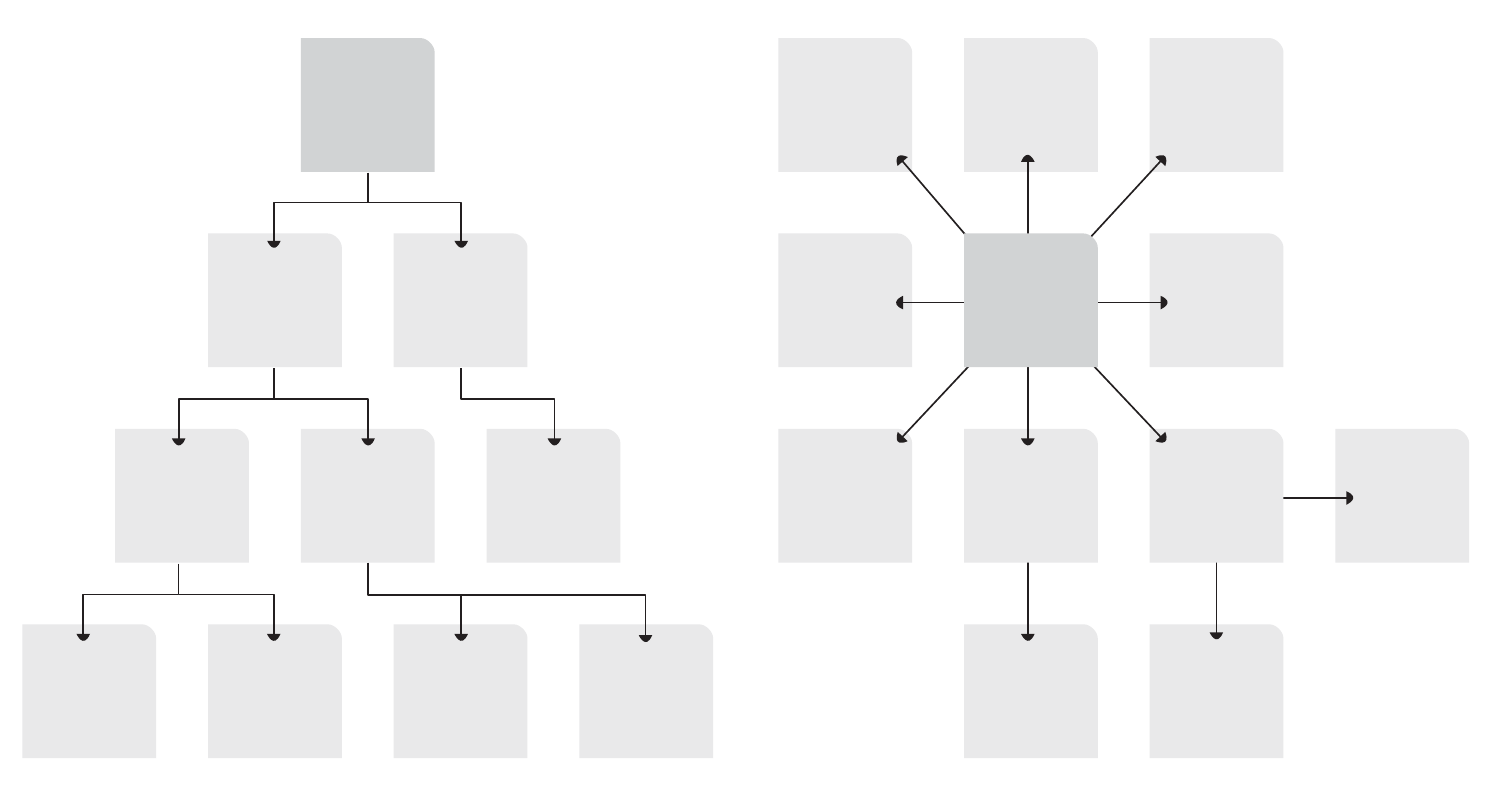
\includegraphics[width=\textwidth]{structure}
 \begin{block}{}
  Слева типичная структура сайта, справа "--- типичная структура приложения
 \end{block}
\end{frame}

\lecturenotes

На следующем этапе разработки необходимо создать общую структуру системы, т. е. выделить отдельные функциональные блоки и определить, как именно эти блоки связываются между собой. Под отдельным функциональным блоком понимается функцию/группу функций, связанных по назначению или области применения в случае приложения и группу функций/фрагментов информационного наполнения в случае сайта.

На слайде представлены типичная структура сайта (слева) и типичная структура приложения. Если сайты обычно разветвлены, в том смысле, что функции обычно размещаются в отдельных экранах, то приложения обычно имеют только один изменяющийся экран, в котором и вызываются почти все функции. Разумеется, это не догма. Проектирование общей структуры состоит из двух параллельно происходящих процессов: выделения независимых блоков и определения связи между ними. Если проектируется сайт, в завершении необходимо также создать схему навигации~\cite[с.~117]{Golovach}.

\begin{frame} \frametitle{Выделение независимых блоков}
 \begin{block}{}
  Не помещайте в один блок больше трех функций.
 \end{block}

 \begin{block}{Пример разделения программы на блоки}
  \begin{itemize}
   \item Основной экран с навигацией между функциями системы.
   \item Создание нового заказа.
   \item Добавление существующего товара в заказ и поиск товара в списке.
   \item Сложный поиск товара.
   \item Добавление нового товара в список.
   \item Обработка заказа, печать и его переход в раздел <<Исполняемые>>.
  \end{itemize}
 \end{block}
\end{frame}

\lecturenotes

Для выделения независимых блоков трудно дать какие-либо конкретные рекомендации, так как очень многое зависит от проектируемой системы. Тем не менее, можно c уверенностью рекомендовать избегать помещения в один блок более трех функций, поскольку каждый блок в результирующей системе будет заключен в отдельный экран или группу управляющих элементов. Перегружать же интерфейс опасно.

Результатом этой работы должен быть список блоков (экранов) с необходимыми пояснениями. пояснениями. В качестве примера рассмотрим гипотетическую программу ввода данных. От пользователя требуется выбрать товары и оформить заказ. При этом блоки разделяются так, как указано на слайде~\cite[с.~117--118]{Golovach}.

\begin{frame} \frametitle{Определение смысловой связи между блоками}

 \begin{block}{Виды связей между блоками}
  \begin{itemize}
   \item Логическая связь определяет взаимодействие между фрагментами системы с точки зрения разработчика.
   \item Связь по представлению пользователей определяет взаимодействие между фрагментами системы с точки зрения пользователей.
   \item Процессуальная связь описывает естественное для имеющегося процесса взаимодействие.
  \end{itemize}
 \end{block}
\end{frame}

\lecturenotes

Существует три основных вида связи между блоками. Это логическая связь, связь по представлению пользователей и процессуальная связь.

Логическая связь определяет взаимодействие между фрагментами системы с точки зрения разработчика (суперпользователя). Важно только помнить, что полученные связи очень существенно влияют на навигацию в пределах системы (особенно, когда система многооконная). Поэтому, чтобы не перегружать интерфейс, стоит избегать как слишком уж отдельных блоков (их трудно найти), так и блоков, связанных с большим количеством других. По моему опыту, для одного блока оптимальным числом связей является число три.

Пользователи имеют свое мнение о системе, и это мнение тоже является важным видом связи. В информационных системах, когда необходимо гарантировать, что пользователь найдет всю нужную ему информацию, необходимо устанавливать связи между блоками, основываясь не только на точке зрения разработчика, но основываясь на представлениях пользователей. 

Наконец, процессуальная связь описывает естественное для имеющегося процесса взаимодействие. Установление качественной процессуальной связи обычно довольно трудная задача, поскольку единственным источником информации является наблюдение за пользователями. Зачем, например, рисовать на экране сложную систему навигации, если точно известно, к какому блоку пользователь перейдет дальше? В этом смысле зачастую оправдано навязывать пользователю какую-либо процессуальную связь, жертвуя удобством, зато выигрывая в скорости обучения (поскольку пользователю приходится думать меньше). Жестко заданная связь позволяет также уменьшить количество ошибок, поскольку от пользователя при ней не требуется спрашивать себя <<не забыл ли я чего?>>. Хорошим примером жестко заданной процессуальной связи является устройство мастеров в Windows, при котором пользователя заставляют нажимать кнопку Далее.

В конце этого этапа должна получиться схема, состоящая из блоков и связей, т.е. переходов между ними~\cite[с.~118--119]{Golovach}.

\subsection{Проектирование отдельных деталей интерфейса}

\begin{frame} \frametitle{Выбор между альтернативными вариантами интерфейса на основе предсказания скорости}
 \begin{block}{Метод GOMS}
  \begin{itemize}
   \item Goals, Operators, Methods, and Selection Rules "--- цели, операторы, методы и правила их выбора.
   \item Разделение действий пользователя на элементарные и суммирование их продолжительности.
   \item Выбор наименьшего по продолжительности варианта.
  \end{itemize}
 \end{block}
 \begin{block}{Недостатки}
  \begin{itemize}
   \item Предсказывает скорость только опытных пользователей.
   \item Не учитывает прогресса пользователей и возможных ошибок.
   \item Плохо применим для сайтов.
  \end{itemize}
 \end{block}
\end{frame}

\lecturenotes

Часто приходится выбирать между разными вариантами реализации интерфейса, причем отбрасывать варианты жалко, потому что они хорошие. Можно, конечно, сделать несколько прототипов и протестировать их на пользователях, но это довольно длительный и трудоемкий процесс. К счастью, есть метод оценки интерфейса, позволяющий быстро выбрать лучший вариант.

В 1983 году Кард, Моран и Ньювел создали метод оценки скорости работы с системой, названный аббревиатурой GOMS (Goals, Operators, Methods, and Selection Rules "--- цели, операторы, методы и правила их выбора).

Идея метода очень проста: все действия пользователя можно разложить на составляющие (например, взять мышь или передвинуть курсор). Ограничив номенклатуру этих составляющих, можно замерить время их выполнения на массе пользователей, после чего получить статистически верные значения длительности этих составляющих. После чего предсказание скорости выполнения какой-либо задачи, или, вернее, выбор наиболее эффективного решения, становится довольно простым делом – нужно только разложить эту задачу на составляющие, после чего, зная продолжительность каждой составляющей, всё сложить и узнать длительность всего процесса. Обычно тот интерфейс лучше, при котором время выполнения задачи меньше.

Впоследствии было разработано несколько более сложных (и точных) вариантов этого метода, но самым распространенным всё равно является изначальный. К сожалению, он имеет определенные недостатки (что, впрочем, уравновешивается его простотой): он применим в основном для предсказания действий опытных пользователей; он никак не учитывает ни прогресса в обучении, ни возможных ошибок, ни степени удовлетворения пользователей; он плохо применим при проектировании сайтов из-за непредсказуемого времени реакции системы~\cite[с.~120--121]{Golovach}.

\begin{frame} \frametitle{Способы улучшить детали интерфейса}
  \begin{itemize}
   \item Адаптивная функциональность.
   \item Принцип масштабируемого интерфейса.
   \item Использование пиктограмм.
  \end{itemize}
\end{frame}

\lecturenotes

Адаптивная функциональность "--- это применение логики, естественной для пользователя. Возьмем пульт от телевизора. Телевизор выключается только одной кнопкой на пульте, но включается от нажатия любой кнопки. Это не следует напрямую из логики системы, но это естественно. Когда на этаж приезжает лифт с неавтоматическими дверями, дверь можно открыть ещё до того, как погаснет кнопка вызова (чтобы лифт не увели). Это не вполне логично, но естественно. Оба примера демонстрируют готовность системы (а точнее, её разработчиков) усложнить свою логику, чтобы упростить логику пользователя. Результат: систему легче использовать. Остается один вопрос: как определить, какие фрагменты и функции системы должны быть адаптивными? Ответ: единственным решением является детальный анализ взаимодействия пользователей с системой. Помочь здесь может только тестирование интерфейса на пользователях.~\cite[с.~124]{Golovach}

Идея масштабируемого интерфейса заключается в том, что пользователь имеет доступ к безграничной плоскости информации с неограниченной степенью разрешения. Эта плоскость является масштабируемой средой и часто изображается как карта. Все, к чему вы можете обратиться, находится где-нибудь на плоскости этой среды. Вы можете находиться на определенной <<высоте>> над ней, поднимаясь <<вверх>> для увеличения масштаба и спускаясь <<вниз>> для уменьшения. Навигация по системе осуществляется как с помощью изменения высоты, так и с помощью поиска.

Пиктограммы делают интерфейс более привлекательным в визуальном отношении и, при определенных условиях, могут способствовать большей понятности. Кроме того, использование пиктограмм позволяет намного упростить процесс перевода программ на другие языки. Однако у пиктограмм есть существенный недостаток. Ее смысл может быть неочевиден, или же ее изображение может дать неверное сообщение для тех, кто с ним незнаком или кем это изображение может быть истолковано по-другому в силу культурных особенностей. В этих случаях пиктограммы рекомендуется заменить на надписи~\cite[с.~115--125]{Raskin}.

\section{Разработка интерфейса, ориентированного на пользователя}

\subsection{Определение user experience и user-centered design}

\begin{frame} \frametitle{Определение user experience и user-centered design}
  \begin{definition}
    \alert{User experience (UX)} "--- это желаемый, ожидаемый или фактический опыт пользователя, взаимодействующего с продуктом.
  \end{definition}
  
  \begin{definition}
    \alert{User-centered design или разработка, ориентированная на пользователя} "--- это процесс разработки интерфейса, на каждом этапе которого существенное внимание уделяется потребностям и ограничениям конечных пользователей продукта.
  \end{definition}
\end{frame}

\lecturenotes

User experience или опыт пользователя "--- это желаемый, ожидаемый или фактический опыт пользователя, взаимодействующего с продуктом.

User-centered design или разработка, ориентированная на пользователя} "--- это процесс разработки интерфейса, на каждом этапе которого существенное внимание уделяется потребностям и ограничениям конечных пользователей продукта~\cite[с.~39--40]{Allen}.

Интерфейс является ориентированным на человека, если он отвечает нуждам человека и учитывает его слабости. Чтобы создать такой интерфейс, необходимо иметь представление о том, как действуют люди и машины. Кроме того, следует развить в себе способность чувствовать те трудности, с которыми сталкиваются люди. И это не всегда просто. Мы настолько привыкли к тому, как работают программы, что соглашаемся принять их методы работы как данность, "--- даже в тех случаях, когда их интерфейсы неоправданно сложны, запутанны, неэкономны и побуждают людей к ошибкам~\cite[с.~8]{Raskin}.

Разработчики применяют данный метод, так как он помогает находить лучшие решения. Изучая конечного пользователя веб-сайта или приложения на каждом этапе процесса проектирования, вы создаете более надежный продукт. При тестировании системы с помощью реальных пользователей вы оцениваете его качество и можете определить, как проект нужно улучшить. Метод разработки, ориентированной на пользователя, помогает создавать правильные продукты и создавать продукты правильно.

Основная идея этого метода "--- получать обратную связь от пользователя как можно чаще. Это итеративный процесс "--- разработчик со временем изменяет программу, чтобы отразить знания, полученные в результате исследований. Каждая последующая итерация приводит к лучшему результату~\cite[с.~40--41]{Allen}.

\subsection{Цикл проектирования интерфейса}

\begin{frame} \frametitle{Этапы проектирования интерфейса}
  \begin{itemize}
   \item Исследование.
   \item Разработка.
   \item Исследование, направленное на тестирование и проверку.
  \end{itemize}
\end{frame}

\lecturenotes

UX-разработка обычно состоит из трех этапов: исследования, непосредственной разработки интерфейса и исследования, направленного на тестирование и проверку результата.

На этапе исследования вы изучаете предметную область и контекст. На основе этих знаний вы будете позднее принимать решения по проекту. Постарайтесь на этом этапе узнать как можно больше о бизнесе и целях клиента, будущих пользователях и конкурентах.

На этапе разработки вы определяете, что будет собой представлять ваш интерфейс и как егь части будут сочетаться друг с другом, в том числе сферу действия продукта, его функциональность и поведение.

На этапе проверки вы определяете, как работает продукт, который создали на этапе разработки, с его целевой аудиторией. За этим этапом обычно следуют дальнейшие раунды разработки и тестирования для решения проблем, которые обязательно появятся в результате тестирования с пользователем~\cite[с.~61--62]{Allen}.

\begin{frame} \frametitle{Преимущества метода разработки, ориентированной на пользователя}
  \begin{itemize}
   \item Более качественный продукт.
   \item Исправление ошибок обходится дешевле.
   \item Меньший риск.
   \item Возможность определить более точный дедлайн.
   \item Исследования ведут к пониманию пользователей и их контекста.
   \item Продукт быстрее выпускается на рынок.
  \end{itemize}
\end{frame}

\lecturenotes

У метода разработки, ориентированной на пользователя, есть несколько преимуществ перед другими подходами.

Более качественный продукт "--- процесс, который преднамеренно взаимодействует с конечными пользователями, очевидно, позволяет получить продукт, соответствующий ожиданиям пользователей и работающий по назначению.

Исправление ошибок обходится дешевле "--- вовлекая пользователей в процесс проектирования, вы узнаете, что не работает, еще на ранних этапах. Исправление каркаса или прототипа обходится во много раз дешевле технического исправления после запуска продукта.

Меньший риск "--- подход, ориентированный на пользователя, обеспечивает обнаружение и исправление проблем на этапе проектирования, а не только после запуска. ПО никогда не может быть действительно законченным, но данный подход позволит разработать продукты с большей отказоустойчивостью.

Возможность определить более точный дедлайн и избежать его смещения "--- процесс, ориентированный на пользователя, сам по себе является динамическим и позволяет решить часть проблем достаточно рано, поэтому у вас будет больше шансов избежать переноса дедлайна и завершить продукт в срок.

Исследования ведут к пониманию пользователей и их контекста "--- подход включает в себя углубленный анализ и исследования пользователей и предметной области, которые раскрывают возможности изучить и дифференцировать аналогичные продукты, чтобы получить конкурентные преимущества. Принятые решения по продукту будут зависеть от фактов, полученных в результате исследования, а не на мнении разработчиков.

Продукт быстрее выпускается на рынок "--- проекты, в которых используется метод в чистом виде, позволяют клиенту решать, как именно они будут реализованы. Этот подход помогает обойти длительные процессы принятия решений на стороне клиента. Когда возникают противоречия во взглядах на проект, именно участие пользователей может стать решающим аргументом для дальнейшей работы над проектом~\cite[с.~62--65]{Allen}.

\section{Методы и инструментальные средства проектирования интерфейсов}

\subsection{Исследование пользовательской аудитории}

\begin{frame} \frametitle{Исследование пользовательской аудитории}
  \begin{block}{Цель исследования}
   Выделить основные поведенческие шаблоны пользователей.
  \end{block}
  
  Необходимо знать:
  \begin{itemize}
   \item Цель пользователей при работе.
   \item Задачи, которые пользователи выполняют, чтобы достичь цели.
   \item Термины предметной области, в которой они работают.
   \item Навыки в использовании аналогичного ПО.
  \end{itemize}
\end{frame}

\lecturenotes

Чтобы приступить к созданию интерфейса, необходимо охарактеризовать типы людей, которые будут пользоваться вашим продуктом. Разумеется, каждая группа пользователей, да и каждый пользователь сам по себе уникален. Тем не менее, общие поведенческие шаблоны можно отделить от человеческих особенностей, в этом и заключается основная цель исследования пользовательской аудитории.

В частности, необходимо узнать, какую цель преследуют пользователи при работе, как они декомпозируют ее на задачи, какими терминами пользуются и какими навыками работы они обладают~\cite[с.~25--26]{Tidvell}.

\begin{frame} \frametitle{Виды исследования пользовательской аудитории}
  \begin{itemize}
   \item Непосредственное наблюдение.
   \item Исследование конкретных случаев.
   \item Опросы.
   \item Искуственные образы.
  \end{itemize}
\end{frame}

\lecturenotes

Существует несколько распространенных видов исследования пользовательской аудитории.

Непосредственное наблюдение подразумевает под собой посещение пользователей на месте их работы и интервью с ними. Можно задавать пользователям вопросы о том, каковы их цели и какие задачи они обычно выполняют. Интервью могут быть структурированы, когда вы задаете заранее разработанные вопросы или не структурированы, когда вы спрашиваете то, что придумываете на ходу. Интервью дают большую степень свободы, оно может быть длинным или коротким, формальным и неформальным, личным или по телефону.

Исследования конкретных случаев дают глубокое и подробное представление о нескольких репрезентативных группах пользователей. Их можно применять для пользователей, раздвигающих границы функциональности ПО, например, если вы хотите обновить интерфейс или функциональность продукта. Такие исследования можно проводить в виде долгосрочных экспериментов по наблюдению, изучая контекст использования.

Письменные опросы позволяют получить информацию сразу от множества пользователей. Но, так как прямого контакта при том нет, теряется множество дополнительной информации: если вы о чем-то не спросите, вы об этом не узнаете.

Метод искуственных образов помогает понять, как полученные данные обработать. Эта техника моделирует пользовательскую аудиторию. Для каждой крупной группы пользователей вы создаете его типичного участника, объединяющего наиболее важные аспекты остальных: цели, задачи, навыки. В ходе разработки вы можете задавать себе вопросы, что бы в данной ситуации сделал пользователь, и отвечать на них с помощью созданной модели~\cite[с.~27--28]{Tidvell}.

\subsection{Разработка прототипа}

\begin{frame} \frametitle{Разработка прототипа}
  \begin{block}{}
   Не полируйте прототип. \rmk{Нужно вынести куда-то после этапов и преимуществ и оформить как предупреждение}
  \end{block}

  \begin{block}{Этапы разработки прототипа}
   \begin{itemize}
   \item Бумажная версия.
   \item Презентация.
   \item Программный прототип.
   \end{itemize}
  \end{block}
  
  \begin{block}{Преимущества прототипа}
   \begin{itemize}
   \item Раннее обнаружение проблем.
   \item Обратная связь.
   \item Минимальные затраты ресурсов.
   \end{itemize}
  \end{block}
\end{frame}

\lecturenotes

При создании прототипа наиболее частой ошибкой является стремление сделать прототип возможно более похожим на результирующую систему. Проблема в том, что в большинстве случаев прототип после тестирования оказывается неправильным. Его приходится переделывать, причем иногда полностью, при этом все инвестированные в прототип ресурсы оказываются выброшенными на ветер. Поэтому всегда правильно делать прототип настолько похожим на результирующую систему, насколько версия прототипа поздняя. Первый прототип стоит делать максимально примитивным. Только после того, как тестирование подтверждает его правильность, стоит делать более детализированный прототип.

Бумажная версия прототипа. Необходимо нарисовать на бумаге все экраны и диалоговые окна (читай – распечатать соответствующие части схемы). Нужно только убедиться, что все интерфейсные элементы выглядят единообразно и сколько-нибудь похоже на реальные. Эта распечатка и является первым прототипом. На нём вполне можно тестировать восприятие системы пользователем и её основную логику.

Польза начального прототипирования на бумаге заключается, во-первых, в исключительной простоте модификации по результатам тестирования, а во-вторых, в возможности безболезненно отлавливать представителей целевой аудитории. Значительно легче лестью и коварством завлечь субъекта к письменному столу, нежели к компьютеру, на котором надо чтото запускать, ждать, пока запустится и так далее.

После исчерпания возможностей бумажной версии прототипа стоит создать новую версию, исправив уже обнаруженные проблемы. Для этого точно так же рисуется интерфейс, но уже не на бумаге, но в какой-либо презентационной программе (MS PowerPoint, например). При этом каждый экран получает отдельный слайд, а результат нажатия кнопок имитируется переходами между слайдами. С этой версией прототипа можно тестировать значительно более сложное взаимодействие человека с системой, нежели с бумажной. С другой стороны, исправление найденных ошибок значительно более трудоемко. Фактически для большинства систем этой версии оказывается достаточно.

В тех случаях, когда в интерфейсе появляются нестандартные элементы или необходимо проверить реальную скорость взаимодействия пользователя с системой, создается еще одна версия прототипа – реально выглядящая, но лишенная каких-либо алгоритмов и, соответственно, не показывающая реальных данных. Делать этот вариант можно как в средах разработки, благо в них есть визуальные инструменты создания интерфейсов, так и в редакторах изображений. Фактически при этом создаются фальшивые снимки экрана, на которых и производят тестирование~\cite[с.~128--130]{Golovach}.

Преимущества прототипа:

Потенциальные проблемы могут быть обнаружены на самом раннем этапе процесса проектирования, до того, как будет написан какой-либо код.

Поддерживается обратная связь между разработчиками и пользователями.
    
Требуются только минимальные ресурсы и материалы. Бумажные прототипы быстро собираются и улучшаются, что позволяет быстро выполнять итерации взаимодействия с пользователями или заказчиками~\cite{Usabilitynet-prototyping}.

\subsection{Инструменты проектирования интерфейса}

\begin{frame} \frametitle{Лучшие инструменты для дизайна и проектирования 2016}
  \begin{itemize}
   \item Векторные и растровые графические редакторы:
     \begin{itemize}
      \item Adobe Photoshop
      \item Sketch
      \item Microsoft Visio
      \item CorelDRAW
      \item Pencil
     \end{itemize}
   \item Средства прототипирования:
     \begin{itemize}
      \item Axure RP
      \item Balsamiq Mockups
      \item InVision
      \item Mockingbird
      \item Proto.io
      \item MockFlow
      \item Flinto 
     \end{itemize}
  \end{itemize}
  
  \url{https://tagline.ru/graphic-ui-ux-design-instruments-rating/}
\end{frame}

Cервисы и инструменты, которые чаще всего используются в дизайне, проектировании и прототипировании: векторные и растровые графические редакторы (Adobe Photoshop, Sketch, Microsoft Visio); средства прототипирования (Axure RP, Balsamiq Mockups, InVision).

Рейтинг инструментов для дизайна и проектирования проводится Тэглайном в третий раз (при поддержке Looi Factory) и сформирован на основе опроса 460+ digital-агентств с производством и/или клиентским офисом в России (с августа 2014 по апрель 2016 года). Респондентам предлагалось ответить на два вопроса: <<Какие инструменты проектирования и прототипирования вы используете в процессе разработки?>> и <<Какие растровые и векторные графические редакторы и утилиты вы используете (помимо средств прототипирования)?>>

Почти все инструменты доступны для Mac OS и Windows, Pencil доступен также для Linux; Adobe Photoshop, Microsoft Visio и Proto.io имеют и Android-версию. Примерно половина из них имеет версию для браузера: Adobe Photoshop, Balsamiq Mockups, InVision, Mockingbird (только браузерная), Proto.io, MockFlow, Flinto.

Все инструменты из рейтинга коммерческие и приобретение их полнофункциональной версии потребует оплаты. Часть инчтрументов имеют бесплатную пробную версию с ограниченной функциональностью: Adobe Photoshop на 7 дней, Proto.io на 15, InVision, MockFlow и Pencil бессрочно~\cite{Rating2016}.

\begin{thebibliography}{99}
\bibitem{Bauman} \href{http://ru.bmstu.wiki/Интерфейс_пользователя}{Национальная библиотека им. Н. Э. Баумана. Интерфейс пользователя.}
\bibitem{Raskin} Раскин Д. Интерфейс: новые направления в проектировании компьютерных систем. СПб.: Символ-Плюс. 2004;272.
\bibitem{Allen} Allen JJ, Chudley JJ. Smashing UX design: Foundations for designing online user experiences. John Wiley \& Sons; 2012 Apr 25.
\bibitem{Golovach} Влад В. Головач. Дизайн пользовательского интерфейса. Искусство мыть слона. 2009.
\bibitem{Tidvell} Тидвелл Д. Разработка пользовательских интерфейсов. Питер; 2011.
\bibitem{Rating2016} \href{https://tagline.ru/graphic-ui-ux-design-instruments-rating/}{Рейтинг инструментов для дизайна и проектирования 2016}
\bibitem{Usabilitynet-prototyping} \href{http://www.usabilitynet.org/tools/prototyping.htm}{Usability Net Paper prototyping}
\bibitem{Usabilitynet-scenarios} \href{http://www.usabilitynet.org/tools/scenarios.htm}{Usability Net Scenarios of use (Use cases)}
\bibitem{Rosenberg} Rosenberg D., Stephens M. Use case driven object modeling with UML //APress, Berkeley, USA. – 2007.
\end{thebibliography}

\end{document}

%%% Local Variables: 
%%% mode: TeX-pdf
%%% TeX-master: t
%%% End: 
